\documentclass{scalatekids-article}
\begin{document}
\lfoot{Analisi dei Requisiti 0.0.1}
\newgeometry{top=3.5cm}
\begin{titlepage}
  \begin{center}
    \begin{center}
      
\includegraphics[width=10cm]{sklogo.png}
    \end{center}
    \vspace{1cm}
    \begin{Huge}
      \begin{center}
        \textbf{Analisi dei Requisiti}
      \end{center}
    \end{Huge}
    \vspace{11pt}
    \bgroup
    \def\arraystretch{1.3}
    \begin{tabular}{r|l}
      \multicolumn{2}{c}{\textbf{Informazioni sul documento}} \\
      \hline
      \setbox0=\hbox{0.0.1\unskip}\ifdim\wd0=0pt
      \\
      \else
      \textbf{Versione} & 0.0.3\\
      \fi
      \textbf{Redazione} & \multiLineCell[t]{Redattore}\\
      \textbf{Verifica} & \multiLineCell[t]{Verificatore}\\
      \textbf{Approvazione} & \multiLineCell[t]{Approvatore}\\
      \textbf{Uso} & Esterno\\
      \textbf{Lista di Distribuzione} & \multiLineCell[t]{ScalateKids\\Prof. Tullio Vardanega\\Prof. Riccardo Cardin}\\
    \end{tabular}
    \egroup
    \vspace{22pt}
  \end{center}
\end{titlepage}
\restoregeometry
\clearpage
\setcounter{page}{1}
\begin{flushleft}
  \vspace{0cm}
         {\large\bfseries Diario delle modifiche \par}
\end{flushleft}
\vspace{0cm}
\begin{center}
  \begin{tabular}{| l | l | l | l | l |}
    \hline
    Versione & Autore & Ruolo & Data & Descrizione \\
    \hline
    0.0.1 & Andrea Giacomo Baldan & & 2015-12-27 & Creazione scheletro del documento\\
    \hline
  \end{tabular}
\end{center}
\tableofcontents
\newpage
\section{Sommario}
\subsection{Scopo del documento}
Il seguente documento ha lo scopo di presentare le funzionalità che il prodotto
\textbf{Actorbase} esporrà all'utilizzatore finale. Inoltre elenca e descrive i
requisiti derivanti dalle suddette funzionalità, emersi durante le riunioni
interne ed esterne con il proponente.
\prodPurpose \glossExpl
\subsection{Riferimenti}
\subsubsection{Normativi}
\begin{itemize}
\item\textbf{Capitolato d'appalto C1:} \textit{Actorbase: a NoSQL DB based on the Actor model}\\
  \url{http://www.math.unipd.it/~tullio/IS-1/2015/Progetto/C1.pdf}
\item\textbf{Verbale esterno:} % TODO link
\item\textbf{Norme di Progetto:} % TODO link
\end{itemize}
\subsubsection{Informativi}
\begin{itemize}
\item\textbf{Dispense fornite dall'insegnamento Ingegneria del Software mod. A:}\\
  \url{http://www.math.unipd.it/~tullio/IS-1/2015/Dispense/L06.pdf}
\item\textbf{Dispense fornite dall'insegnamento Ingegneria del Software mod. A:}\\
  \url{http://www.math.unipd.it/~tullio/IS-1/2015/Dispense/E02.pdf}
\item\textbf{CAP theorem:}\\ % TODO: da inserire?
  \url{https://en.wikipedia.org/wiki/CAP_theorem}
\item\textbf{Reactive Manifesto:}
  \url{http://www.reactivemanifesto.org/}
  \url{https://en.wikipedia.org/wiki/Reactive_programming}
\item\textbf{Amazon DynamoDB:}
  \url{http://docs.aws.amazon.com/amazondynamodb/latest/developerguide/Introduction.html}
\end{itemize}
\section{Descrizione generale}
\subsection{Prospettive del prodotto}
l'obiettivo del prodotto è fornire un database \gloss{NoSQL} di tipo
\gloss{key-value}, quindi senza schemi predefiniti e tabelle; che utilizzi il
modello ad attori per garantire un alto grado di \gloss{concorrenza} e
\gloss{scalabilità orizzontale} idealmente illimitata.
\subsection{Funzioni}
Il software fornirà un sistema di interazione con l'utente basata su \gloss{ui}
testuale direttamente da riga di comando. Permetterà di effettuare le operazioni
basilari che ogni database fornisce:
\begin{itemize}
\item Creazione di una o più collezioni;
\item Cancellazione di una o più collezioni;
\item Modifica di una collezione;
\item Ricerca all'interno del database o all'interno di una o più collezioni;
\item Inserimento;
\item Cancellazione;
\item Aggiornamento;
\item Importazione ed esportazione di dati in formato \gloss{JSON}. % TODO: controllare
\end{itemize}
Il programma inoltre permetterà la richiesta di un aiuto esplicativo sull'uso
dei comandi.
\subsection{Caratteristiche utenza}
Il prodotto è orientato all'utilizzo da parte di clientela interessata a
sviluppo di applicazioni \gloss{reactive}, che trattino grandi moli di dati e
debbano fornire brevissimi tempi di risposta, sacrificando dunque le
funzionalità relazionali tipiche dei tradizionali database \textit{SQL} in
favore di un sistema fortemente \gloss{concorrente} e senza l'\gloss{overhead} generato
dagli schemi \gloss{SQL}.
\subsection{Vincoli}
Per far funzionare \textbf{Actorbase} è necessario disporre di un computer con
installata la \textit{\gloss{JVM} versione 8}. Non ci sono ulteriori richieste h
ardware o software.
\section{Casi d'uso}
Le aspettative di esperienza utente derivano dall'utilizzo da parte dei
componenti del gruppo di \gloss{Amazon DynamoDB}, un database \gloss{key-value}
sviluppato da \textit{Amazon}, utilizzato come modello di riferimento per lo
sviluppo. I casi d'uso seguono le norme di stesura elencate nel documento \textit{Norme di Progetto}.% TODO link
\subsection{UC1: Actorbase}
\begin{center}
  \begin{figure}[H]
    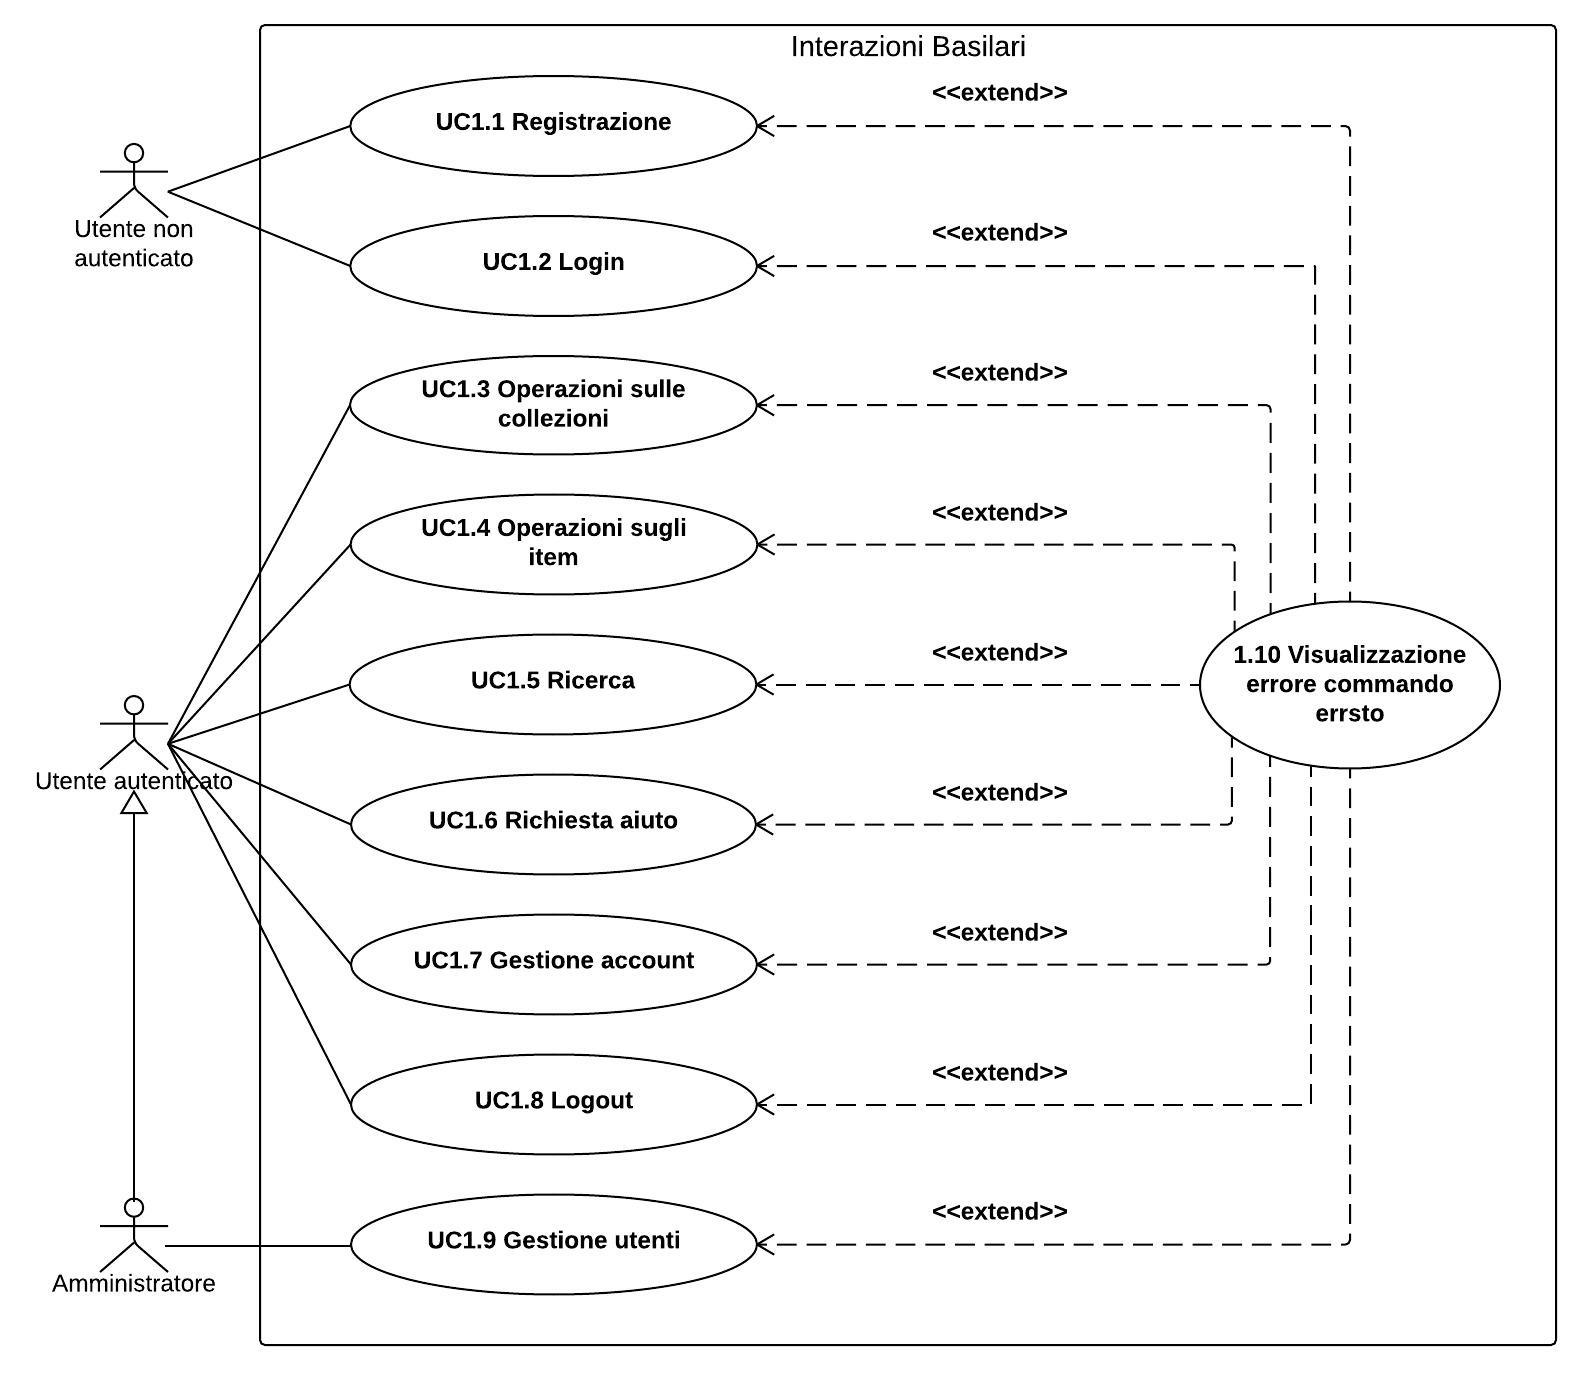
\includegraphics[width=0.7\textwidth,keepaspectratio]{UseCases/InterazioniBasilari.jpeg}
    \caption{Caso d'uso 1: Interazioni basilari}
  \end{figure}
\end{center}
\textbf{Attori primari:} Utente non autenticato, Utente autenticato, Amministratore\\ \\
\textbf{Scopo e descrizione:}
L’utente ha appena avviato la \gloss{CLI}, risulta essere non autenticato, può quindi
registrarsi, oppure, se è già registrato, può effettuare il login diventando utente
autenticato. Le operazioni che può eseguire a login effettuato sono:
\begin{itemize}
\item Gestire il proprio \gloss{account};
\item Operazioni sulle collezioni;
\item Operazioni sugli \gloss{item};
\item Ricerca;
\item Richiedere aiuto;
\item Effettuare il logout.
\end{itemize}
Nel caso in cui si tratti di un amministratore, oltre alle operazioni elencate, può effettuare operazioni di gestione sugli utenti
esistenti nel database.
\textbf{Precondizione:} Il database è installato correttamente, e il server è in ascolto.\\ \\
\textbf{Flusso eventi:}
\begin{itemize}
\item UC1.1 Registrazione;
\item UC1.2 Login;
\item UC1.3 Operazioni sulle collezione;
\item UC1.4 Operazioni sugli \gloss{item};
\item UC1.5 Ricerca;
\item UC1.6 Richiesta aiuto;
\item UC1.7 Gestione account;
\item UC1.8 Effettuare il logout;
\item UC1.9 Gestione utenti.
\end{itemize}
\textbf{Postcondizione:} Il sistema ha prodotto l'output corrispondente al comando immesso dall'utente.
\subsection{UC1.1: Registrazione}
\textbf{Attore primario:} Utente non autenticato\\ \\
\textbf{Scopo e descrizione:} L'utente intende accedere al sistema \textbf{Actorbase}. Per farlo necessita di un
profilo registrato all'interno del programma. Deve registrare un nome utente e una password.\\ \\
\textbf{Precondizione:} L'utente non è registrato e richiede la registrazione.\\ \\
\textbf{Flusso eventi:}
\begin{itemize}
\item Inserimento username;
\item Inserimento password;
\item Conferma password.
\end{itemize}
\textbf{Estensioni:}
\begin{itemize}
\item Nel caso in cui l'utente utilizzi un comando sconosciuto:
  \begin{itemize}
  \item viene visualizzato un messaggio di errore esplicativo (e rimando all'aiuto);
  \end{itemize}
\item Nel caso in cui l'utente utilizzi un comando conosciuto ma con parametri errati:
  \begin{itemize}
  \item viene visualizzato un messaggio di supporto che indica come usare correttamente il comando.
  \end{itemize}
\item Nel caso in cui l'username inserito sia già presente all'interno del sistema:
  \begin{itemize}
  \item viene visualizzato un messaggio di errore esplicativo.
  \end{itemize}
\end{itemize}
\textbf{Postcondizione:} L'utente è registrato all'interno del sistema \textbf{Actorbase}.
\subsection{UC1.2: Login}
\textbf{Attore primario:} Utente non autenticato\\ \\
\textbf{Scopo e descrizione:} L’utente già registrato, intende accedere al sistema \textbf{Actorbase}. Deve inserire le proprie credenziali di accesso. \\ \\
\textbf{Flusso di eventi:}
\begin{itemize}
\item Inserimento username;
\item Inserimento password.
\end{itemize}
\textbf{Estensioni:}
\begin{itemize}
\item Nel caso in cui l'utente utilizzi un comando sconosciuto:
  \begin{itemize}
  \item viene visualizzato un messaggio di errore esplicativo (e rimando all'aiuto);
  \end{itemize}
\item Nel caso in cui l'utente utilizzi un comando conosciuto ma con parametri errati:
  \begin{itemize}
  \item viene visualizzato un messaggio di supporto che indica come usare correttamente il comando.
  \end{itemize}
\end{itemize}
\textbf{Postcondizione:} L'utente è autenticato all'interno del sistema \textbf{Actorbase}.
\subsection{UC1.3: Richiesta aiuto}
\textbf{Attore primario:} Utente autenticato\\ \\
\textbf{Scopo e descrizione:} L'utente intende richiedere aiuto generale o su un comando specifico.\\ \\
\textbf{Precondizione:} Il database è pronto a ricevere comandi e l'utente intende richiedere supporto.\\ \\
\textbf{Flusso di eventi:}
\begin{itemize}
\item UC1.3.1 Inserimento comando per richiesta aiuto generale;
\item UC1.3.1 Inserimento comando per aiuto specifico.
\end{itemize}
\textbf{Postcondizione:} Il sistema ha risposto con l'aiuto richiesto in output.
\subsection{UC1.6.1: Richiesta di aiuto generale}
\textbf{Attore primario:} Utente autenticato\\ \\
\textbf{Scopo e descrizione:} L'utente intende richiedere aiuto generale sull'utilizzo del sistema \textbf{Actorbase}.\\ \\
\textbf{Precondizione:} Il database è pronto a ricevere comandi e l'utente intende richiedere supporto.\\ \\
\begin{itemize}
\item Inserimento comando per aiuto.
\end{itemize}
\textbf{Postcondizione:} Il sistema ha risposto con l'aiuto richiesta in output.
\subsection{UC1.3.2: Richiesta di aiuto specifico}
\textbf{Attore primario:} Utente autenticato\\ \\
\textbf{Scopo e descrizione:} L'utente intende richiedere aiuto su uno specifico comando del sistema \textbf{Actorbase}.\\ \\
\textbf{Flusso di eventi:}
\begin{itemize}
\item inserimento comando per aiuto;
\item Inserimento nome comando.
\end{itemize}
\textbf{Postcondizione:} Il sistema ha risposto con l'aiuto richiesto in output.
\subsection{UC1.4: Operazioni sulle collezioni}
\textbf{Attore primario:} Utente autenticato\\ \\
\textbf{Scopo e descrizione:} L'utente è autenticato e desidera effettuare delle operazioni sulle collezioni. Le operazioni previste sono
creazione di una nuova collezione, elencazione delle collezioni esistenti, cancellazione di collezioni esistenti, modifica del nome di collezioni esistenti,
aggiunta o rimozione collaboratori a collezione esistente.\\ \\
\textbf{Precodizione:} Il database è pronto a ricevere comandi e l'utente intende effettuare operazioni su collezioni.\\ \\
\textbf{Flusso di eventi:}
\begin{itemize}
\item UC1.4.1 Creazione nuova collezione;
\item UC1.4.2 Elencazione collezioni;
\item UC1.4.3 Cancellazione collezioni;
\item UC1.4.6 Modifica nome collezione;
\item UC1.4.4 Aggiunta collaboratore;
\item UC1.4.5 Rimozione collaboratore.
\end{itemize}
\textbf{Estensioni:}
\begin{itemize}
\item Nel caso in cui l'utente utilizzi un comando sconosciuto:
  \begin{itemize}
  \item viene visualizzato un messaggio di errore esplicativo (e rimando all'aiuto);
  \end{itemize}
\item Nel caso in cui l'utente utilizzi un comando conosciuto ma con parametri errati:
  \begin{itemize}
  \item viene visualizzato un messaggio di supporto che indica come usare correttamente il comando.
  \end{itemize}
\item Nel caso in cui il nome di una collezione sia già utilizzato:
  \begin{itemize}
  \item viene visualizzato un messaggio di errore esplicativo;
  \end{itemize}
\item Nel caso in cui la collezione da cancellare o modificare non sia presente:
  \begin{itemize}
  \item viene visualizzato un messaggio di errore esplicativo;
  \end{itemize}
\item Nel caso in cui il collaboratore da rimuovere non sia presente tra i collaboratori:
  \begin{itemize}
  \item viene visualizzato un messaggio di errore esplicativo;
  \end{itemize}
\item Nel caso in cui il collaboratore da aggiungere non sia presente nel sistema \textbf{Actorbase}:
  \begin{itemize}
  \item viene visualizzato un messaggio di errore esplicativo;
  \end{itemize}
\end{itemize}
\textbf{Postcondizione:} L'operazione richiesta è stata eseguita.
\subsection{UC1.4.1: Creazione nuova collezione}
\textbf{Attore primario:} Utente autenticato\\ \\
\textbf{Scopo e descrizione:} L'utente richiede la creazione di una collezione all'interno del database, deve inserire il nome della nuova collezione.\\ \\
\textbf{Precodizione:} Il database è pronto a ricevere comandi e l'utente intende creare una collezione.\\ \\
\textbf{Flusso di eventi:}
\begin{itemize}
\item Inserimento nome collezione
\end{itemize}
\textbf{Postcondizione:} La collezione è stata creata.
\subsection{UC1.4.2: Elencazione collezioni}
\textbf{Attore primario:} Utente autenticato\\ \\
\textbf{Scopo e descrizione:} L'utente intende elencare tutte le collezioni all'interno di \textbf{Actorbase} secondo la propria visibilità.\\ \\
\textbf{Precodizione:} Il database è pronto a ricevere comandi e l'utente intende elencare le collezioni al suo interno.\\ \\
\textbf{Postcondizione:} Il database restituisce la lista delle collezioni esistenti secondo la visibilità dell'utente.
\subsection{UC1.4.3: Cancellazione di una o più collezioni}
\textbf{Attore primario:} Utente autenticato\\ \\
\textbf{Scopo e descrizione:} L’utente intende cancellare una o più collezioni presenti nel database.\\ \\
\textbf{Precodizione:} Il database è pronto a ricevere comandi e l’utente intende cancellare una o più collezioni\\ \\
\textbf{Flusso di eventi:}
\begin{itemize}
\item Inserimento di una o più nomi di collezioni da cancellare.
\end{itemize}
\textbf{Postcondizione:} Le collezioni sono state rimosse dal database.
\subsection{UC1.4.4: Modifica nome collezione}
\textbf{Attore primario:} Utente autenticato \\ \\
\textbf{Scopo e descrizione:} L’utente intende modificare il nome di una collezione, deve inserire il nome della collezion da modificare e il nuovo nome da assegnare. \\ \\
\textbf{Precondizione:} Il database è pronto a ricevere comandi e l’utente intende modificare il nome di una collezione\\ \\
\textbf{Flusso di eventi:}
\begin{itemize}
\item Inserimento nome della collezione da modificare;
\item Inserimento nuovo nome della collezione.
\end{itemize}
\textbf{Postcondizione:} Il nome della collezione è stato modificato
\subsection{UC1.4.5: Aggiunta di un collaboratore a propria collezione}
\textbf{Attore primario:} Utente autenticato\\ \\
\textbf{Scopo e descrizione:} L'utente intende aggiungere un collaboratore ad una collezione di sua proprietà. Deve inserire il nome della collezione e lo username dell'utente da aggiungere.\\ \\
\textbf{Precondizione:} Il database è pronto a ricevere comandi e l'utente intende aggiungere un collaboratore ad una collezione di sua proprietà.\\ \\
\textbf{Flusso di eventi:}
\begin{itemize}
\item Inserimento nome collezione;
\item Inserimento username collaboratore.
\end{itemize}
\textbf{Postcondizione:} L'utente designato per la collaborazione è stato aggiunto tra i collaboratori della collezione scelta.
\subsection{UC1.4.6: Rimozione di un collaboratore a propria collezione}
\textbf{Attore primario:} Utente autenticato\\ \\
\textbf{Scopo e descrizione:} L'utente intende rimuovere un collaboratore da una collezione di sua proprietà. Deve inserire il nome della collezione e lo username del collaboratore da rimuovere.\\ \\
\textbf{Precondizione:} Il database è pronto a ricevere comandi e l'utente intende rimuovere un collaboratore da una collezione di sua proprietà.\\ \\
\textbf{Flusso di eventi:}
\begin{itemize}
\item Inserimento nome collezione;
\item Inserimento username collaboratore.
\end{itemize}
\textbf{Postcondizione:} L'utente designato per la rimozione dai collaboratori è stato rimosso dalla collezione scelta.
\subsection{UC1.5: Operazioni sugli \gloss{item}}
\textbf{Attore primario:} Utente autenticato\\ \\
\textbf{Scopo e descrizione:} L'utente intende effettuare operazioni sugli item di una collezione esistente. Le operazioni previste sono:
inserimento e cancellazione.\\ \\
\textbf{Precondizione:} Il database è pronto a ricevere comandi e l'utente intende effettuare operazioni di inserimento o cancellazione su una collezione esistente.\\ \\
\textbf{Flusso di eventi:}
\begin{itemize}
\item UC1.5.1 Inserimento nuovo item;
\item UC1.5.2 Cancellazione item.
\end{itemize}
\textbf{Estensioni:}
\begin{itemize}
\item Nel caso in cui l'utente utilizzi un comando sconosciuto:
  \begin{itemize}
  \item viene visualizzato un messaggio di errore esplicativo (e rimando all'aiuto);
  \end{itemize}
\item Nel caso in cui l'utente utilizzi un comando conosciuto ma con parametri errati:
  \begin{itemize}
  \item viene visualizzato un messaggio di supporto che indica come usare correttamente il comando.
  \end{itemize}
\item Nel caso in cui la collezione su cui effettuare inserimento o cancellazione non sia presente:
  \begin{itemize}
  \item viene visualizzato un messaggio di errore esplicativo;
  \end{itemize}
\end{itemize}
\textbf{Postcondizione:} L'operazione richiesta è stata effettuata correttamente.
\subsection{1.5.1 Inserimento nuovo item}
\textbf{Attore primario:} Utente autenticato\\ \\
\textbf{Scopo e descrizione:} L'utente intende inserire un nuovo item all'interno di una collezione esistente. Deve selezionare la collezione e inserire i parametri di definizione dell'item. Questi sono la chiave e il valore associato.\\ \\
\textbf{Precondizione:} Il database è pronto a ricevere comandi e l'utente intende effetture un inserimento di un nuovo item.\\ \\
\textbf{Flusso di eventi:}
\begin{itemize}
\item UC1.5.1.1 Inserimento con sovrascrittura;
\item UC1.5.1.2 Inserimento senza sovrascrittura.
\end{itemize}
\textbf{Postcondizione:} L'operazione di inserimento richiesta è stata effettuata correttamente.
\subsection{1.5.1.1 Inserimento con sovrascrittura (aggiornamento)}
\textbf{Attore primario:} Utente autenticato\\ \\
\textbf{Scopo e descrizione:} L'utente intende inserire un nuovo item; deve selezionare la collezione e inserire i parametri di definizone dell'item da inserire, quali chiave e valore associato. La procedura di inserimento non terrà conto di
eventuali chiavi già presenti all'interno della collezione\\ \\
\textbf{Precondizione:} Il database è pronto a ricevere comandi e l'utente intende effettuare un inserimento di un nuovo item.\\ \\
\textbf{Flusso di eventi:}
\begin{itemize}
\item Inserimento nome collezione su cui effettuare l'inserimento;
\item Inserimento coppia chiave-valore da inserire.
\end{itemize}
\textbf{Postcondizione:} L'operazione di inserimento con sovrascrittura è andata a buon fine, eventuali chiavi già presenti avranno i valori associati aggiornati.
\subsection{1.5.1.2 Inserimento senza sovrascrittura}
\textbf{Attore primario:} Utente autenticato \\ \\
\textbf{Scopo e descrizione:} L'utente intende inserire un nuovo item; deve selezionare la collezione e inserire i parametri di definizione dell'item da inserire, quali chiave e valore associato. La procedura di inserimento terrà conto di chiavi già presenti all'interno della collezione selezionata.\\ \\
\textbf{Precondizione:} Il database è pronto a ricevere comandi e l'utente intende effettuare un inserimento di un nuovo item.\\ \\
\textbf{Flusso di eventi:}
\begin{itemize}
\item Inserimento nome collezione su cui effettuare l'inserimento;
\item Inserimento coppia chiave-valore da inserire.
\end{itemize}
\textbf{Estensioni:}
\begin{itemize}
\item Nel caso in cui la chiave scelta sia già presente all'interno della collezione:
  \begin{itemize}
  \item viene visualizzato un messaggio di errore esplicativo;
  \end{itemize}
\end{itemize}
\textbf{Postcondizione:} L'operazione di inserimento senza sovrascrittura è andata a buon fine.
\subsection{UC1.5.1 Cancellazione di un item}
\textbf{Attore primario:} Utente autenticato\\ \\
\textbf{Scopo e descrizione:} L'utente intende cancellare un item all'interno di una collezione esistente. Deve selezionare la collezione e inserire la chiave da del valore da cancellare.\\ \\
\textbf{Precondizione:} Il database è pronto a ricevere comandi e l'utente intende effetture la cancellazione di un item.\\ \\
\textbf{Flusso di eventi:}
\begin{itemize}
\item Inserimento nome collezione;
\item Inserimento chiave.
\end{itemize}
\subsection{UC1.6: Ricerca generale}
\textbf{Attore primario:} Utente autenticato \\ \\
\textbf{Scopo e descrizione:} L’utente intende effettuare una ricerca, può decidere se effettuare la ricerca a livello globale nella base di dati o solo su una lista di collezioni scelte.\\ \\
\textbf{Precondizione:} Il database è pronto a ricevere comandi e l’utente intende effettuare una ricerca\\ \\
\textbf{Flusso di eventi:}
\begin{itemize}
\item UC1.6.1 Ricerca sull'intera base di dati;
\item UC1.6.2 Ricerca su una o più collezioni.
\end{itemize}
\begin{itemize}
\item Nel caso in cui l'utente utilizzi un comando sconosciuto:
  \begin{itemize}
  \item viene visualizzato un messaggio di errore esplicativo (e rimando all'aiuto);
  \end{itemize}
\item Nel caso in cui l'utente utilizzi un comando conosciuto ma con parametri errati:
  \begin{itemize}
  \item viene visualizzato un messaggio di supporto che indica come usare correttamente il comando.
  \end{itemize}
\item Nel caso in cui la collezione su cui effettuare ricerca non sia presente:
  \begin{itemize}
  \item viene visualizzato un messaggio di errore esplicativo;
  \end{itemize}
\end{itemize}
\textbf{Postcondizione:} Il sistema ha prodotto in output i risultati della ricerca effettuata.
\subsection{UC1.6.1: Ricerca all'interno della base di dati}
\textbf{Attore primario:} Utente autenticato \\ \\
\textbf{Scopo e descrizione:} L’utente intende effettuare una ricerca sull’intera base di dati, deve inserire i parametri di ricerca.\\ \\
\textbf{Precondizione:} Il database è pronto a ricevere comandi e l’utente intende effettuare una ricerca generale\\ \\
\textbf{Flusso di eventi:}
\begin{itemize}
\item Inserimento parametri di ricerca.
\end{itemize}
\textbf{Postcondizione:} Il sistema ha prodotto in output i risultati della ricerca effettuata.
\subsection{UC1.6.2: Ricerca all'interno di una specifica collezione(o più)}
\textbf{Attore primario:} Utente autenticato \\ \\
\textbf{Scopo e descrizione:} L’utente intende effettuare una ricerca all’interno di una o più collezioni specifiche, deve inserire le collezioni su cui effettuare la ricerca e i parametri di ricerca.\\ \\
\textbf{Precondizione:} Il database è pronto a ricevere comandi e l’utente intende effettuare una ricerca dettagliata\\ \\
\textbf{Flusso di eventi:}
\begin{itemize}
\item Inserimento nomi collezioni;
\item Inserimento parametri di ricerca.
\end{itemize}
\textbf{Postcondizione:} Il sistema ha prodotto in output i risultati della ricerca effettuata.
\subsection{UC1.7: Gestione account}
\textbf{Attore primario:} Utente autenticato\\ \\
\textbf{Scopo e descrizione:} L'utente intende effettuare operazioni di gestione sul proprio account. Le operazioni previste sono
Modifica username e modifica password.\\ \\
\textbf{Precondizione:} Il database è pronto a ricevere comandi e l'utente intende effettuare operazioni di gestione del proprio account.\\ \\
\textbf{Flusso di eventi:}
\begin{itemize}
\item UC1.7.1 Modifica username;
\item UC1.7.2 Modifica password.
\end{itemize}
\textbf{Estensioni:}
\begin{itemize}
\item Nel caso in cui l'utente utilizzi un comando sconosciuto:
  \begin{itemize}
  \item viene visualizzato un messaggio di errore esplicativo (e rimando all'aiuto);
  \end{itemize}
\item Nel caso in cui l'utente utilizzi un comando conosciuto ma con parametri errati:
  \begin{itemize}
  \item viene visualizzato un messaggio di supporto che indica come usare correttamente il comando.
  \end{itemize}
\item Nel caso in cui il nuovo username scelto sia già presente nel sistema \textbf{Actorbase}:
  \begin{itemize}
  \item viene visualizzato un messaggio di errore esplicativo;
  \end{itemize}
\end{itemize}
\textbf{Postcondizione:} L'operazione richiesta è andata a buon fine.
\subsection{UC1.8: Logout}
\textbf{Attore primario:} Utente autenticato\\ \\
\textbf{Scopo e descrizione:} L'utente intende effettuare il logout dal sistema \textbf{Actorbase}.\\ \\
\textbf{Precondizione:} Il database è pronto a ricevere comandi e l'utente intende effettuare il logout dal sistema.\\ \\
\textbf{Flusso di eventi:}
\begin{itemize}
\item Inserimento comando di logout.
\end{itemize}
\textbf{Estensioni:}
\begin{itemize}
\item Nel caso in cui l'utente utilizzi un comando sconosciuto:
  \begin{itemize}
  \item viene visualizzato un messaggio di errore esplicativo (e rimando all'aiuto);
  \end{itemize}
\end{itemize}
\textbf{Postcondizione:} L'utente è deautenticato dal sistema \textbf{Actorbase}.
\subsection{UC1.9: Gestione utenti}
\textbf{Attore primario:} Amministratore\\ \\
\textbf{Scopo e descrizione:} L'amministratore intende effettuare operazioni di gestione sugli utenti del database.\\ \\
\textbf{Precondizione:} Il database è pronto a ricevere comandi e l'amministratore intende effettuare operazioni di gestione sugli utenti del sistema.\\ \\
\textbf{Flusso di eventi:}
\begin{itemize}
\item UC1.9.1: Aggiunta nuovo utente;
\item UC1.9.2: Rimozione utente esistente.
\end{itemize}
\textbf{Estensioni:}
\begin{itemize}
\item Nel caso in cui l'amministratore utilizzi un comando sconosciuto:
  \begin{itemize}
  \item viene visualizzato un messaggio di errore esplicativo (e rimando all'aiuto);
  \end{itemize}
\item Nel caso in cui l'amministratore utilizzi un comando conosciuto ma con parametri errati:
  \begin{itemize}
  \item viene visualizzato un messaggio di supporto che indica come usare correttamente il comando.
  \end{itemize}
\item Nel caso in cui il username scelto sia già presente nel sistema \textbf{Actorbase}:
  \begin{itemize}
  \item viene visualizzato un messaggio di errore esplicativo;
  \end{itemize}
\item Nel caso in cui l'utente designato per la rimozione non sia presente nel sistema \textbf{Actorbase}:
  \begin{itemize}
  \item viene visualizzato un messaggio di errore esplicativo;
  \end{itemize}
\end{itemize}
\textbf{Postcondizione:} L'operazione di gestione richiesta è andata a buon fine.
\subsection{UC1.9.1: Aggiunta nuovo utente}
\textbf{Attore primario:} Amministratore\\ \\
\textbf{Scopo e descrizione:} L'amministratore intende aggiungere un nuovo utente al sistema \textbf{Actorbase}.
\textbf{Precondizione:} Il database è pronto a ricevere comandi e l'amministratore intende aggiungere un nuovo utente al sistema.\\ \\
\textbf{Flusso di eventi:}
\begin{itemize}
\item Inserimento username nuovo utente;
\item Inserimento password nuovo utente.
\end{itemize}
\textbf{Postcondizione:} Il nuovo utente designato per l'aggiunta è presente all'interno del sistema \textbf{Actorbase}.
\subsection{UC1.9.1: Rimozione utente esistente}
\textbf{Attore primario:} Amministratore\\ \\
\textbf{Scopo e descrizione:} L'amministratore intende rimuovere un utente esistente dal sistema \textbf{Actorbase}.
\textbf{Precondizione:} Il database è pronto a ricevere comandi e l'amministratore intende rimuovere un utente esistente dal sistema.\\ \\
\textbf{Flusso di eventi:}
\begin{itemize}
\item Inserimento username utente;
\end{itemize}
\textbf{Postcondizione:} L'utente designato per la rimozione non è presente all'interno del sistema \textbf{Actorbase}.
\subsection{UC1.10: Visualizzazione errore}
\textbf{Attore primario:} Utente \\ \\
\textbf{Scopo e descrizione:} L'utente ha inserito un comando errato o ha effettuato un operazione non permessa. Viene visualizzato un messaggio di errore esplicativo specifico, contestualizzato al caso di errore.\\ \\
\textbf{Precondizione:} L'utente ha inserito un comando errato o ha provato ad effettuare un operazione non permessa.\\ \\
\textbf{Flusso di eventi:}
\begin{itemize}
\item UC1.10.1 Errore scrittura comando;
\item UC1.10.2 Errore di timeout;
\item UC1.10.3 Errore di contesto.
\end{itemize}
\textbf{Postcondizione:} Il sistema ha prodotto in output il messaggio di errore, l'operazione che lo ha generato è stata annullata.
\subsection{UC1.10.1: Errore di scrittura comando}
\textbf{Attore primario:} Utente \\ \\
\textbf{Scopo e descrizione:} L'utente ha inserito un comando errato, il sistema non riconosce il comando.\\ \\
\textbf{Precondizione:} L'utente ha inserito un comando errato.\\ \\
\textbf{Flusso di eventi:}
\begin{itemize}
\item Inserimento comando errato.
\end{itemize}
\textbf{Postcondzione:} Il sistema ha prodotto in output il messaggio di errore, l'operazione che lo ha generato è stata annullata.
\subsection{UC1.10.2: Errore di timeout}
\textbf{Attore primario:} Utente \\ \\
\textbf{Scopo e descrizione:} L'utente ha inserito un comando, il tempo di risposta da parte del sistema ha superato una soglia prefissata.\\ \\
\textbf{Precondizione:} L'operazione richiesta dall'utente sta richiedendo un tempo di risposta troppo elevato.\\ \\
\textbf{Flusso di eventi:}
\begin{itemize}
\item Inserimento comando.
\end{itemize}
\textbf{Postcondzione:} Il sistema ha prodotto in output il messaggio di errore, l'operazione che lo ha generato è stata annullata.
\subsection{UC1.10.3: Errore di contesto}
\textbf{Attore primario:} Utente \\ \\
\textbf{Scopo e descrizione:} L'utente ha tentato un operazione non permessa o impossibile da soddisfare.\\ \\
\textbf{Precondizione:} L'utente ha tentato un operazione non permessa o impossibile da soddisfare.\\ \\
\textbf{Flusso di eventi:}
\begin{itemize}
\item Inserimento comando.
\end{itemize}
\textbf{Postcondzione:} Il sistema ha prodotto in output il messaggio di errore nel contesto, l'operazione che lo ha generato è stata annullata.

\subsection{Requisiti funzionali}
\begin{longtable}[H]
\centering
\caption{Tabella requisiti funzionali}
\begin{tabular}{|c|c|c|c|}
\hline
\textbf{Requisito} & \textbf{Tipologia} & \textbf{Descrizione} & \textbf{Fonti}\\
\hline
RF0.21 & \multiLineCell{Tecnologico\\Desiderabile} & y & \multiLineCell{Capitolato\\miniotta\\}\\
\hline
\end{longtable}sadasd & \multiLineCell{Funzionale\\Obbligatorio} & dsa & \multiLineCell{Capitolato\\miniotta\\}\\
\hline
\end{longtable}\subsection{Tracciamento Requisiti-Fonti}
\begin{longtable}[H]
\centering
\caption{Tabella Requisiti-Fonti}
\begin{tabular}{|c|c|}
\hline
\textbf{Requisito} & \textbf{Fonti}\\
\hline
RF0.21 & \multiLineCell[t]{Capitolato\\miniotta\\}\\
\hline
sadasd & \multiLineCell[t]{Capitolato\\miniotta\\}\\
\hline
\end{tabular}
\end{longtable}
\subsection{Tracciamento Fonti-Requisiti}
\begin{longtable}[H]
\centering
\caption{Tabella Fonti-Requisiti}
\begin{tabular}{|c|c|}
\hline
\textbf{Fonte} & \textbf{Requisiti}\\
\hline
Capitolato & \multiLineCell[t]{RF0.21\\sadasd\\}\\
\hline
miniotta & \multiLineCell[t]{RF0.21\\sadasd\\}\\
\hline
\end{tabular}
\end{longtable}
\end{document}
